\documentclass[10pt,a4paper]{article}
\usepackage[utf8]{inputenc}
\usepackage[T1]{fontenc}
\usepackage[spanish,es-noshorthands,es-tabla]{babel}
\usepackage{lmodern,microtype,graphicx,booktabs,tabularx}
\usepackage[table]{xcolor}
\usepackage[margin=0.95cm,top=0.65cm,bottom=0.65cm]{geometry}
\usepackage{hyperref}
\definecolor{azul}{HTML}{14334B}
\definecolor{acento}{HTML}{006699}
\definecolor{suave}{HTML}{EAF3F8}
\definecolor{gris}{HTML}{4A5560}
\hypersetup{colorlinks=true,urlcolor=acento,linkcolor=acento}
\pagestyle{empty}
\setlength{\parindent}{0pt}
\setlength{\parskip}{2pt}
\newcommand{\seccion}[1]{\par\vspace{3pt}{\color{azul}\bfseries\fontsize{10}{11}\selectfont #1}\par\vspace{1pt}}
\newcommand{\rol}[1]{{\color{azul}\bfseries #1}}
\newcommand{\REPO}{https://github.com/Pacortes2021/GENERATIVE-ARTIFICIAL-INTELLIGENCE-DELIVERABLE-1/tree/main/D3\%20alvaro}
\begin{document}
{\color{azul}\bfseries\fontsize{14}{16}\selectfont Agentes para consultas de normativa de pregrado}\par
{\color{acento}\bfseries\fontsize{10}{12}\selectfont Ingeniería UdeC $\cdot$ Entregable 3 $\cdot$ Arquitectura, decisiones y ablaciones de v6}\par
{\fontsize{8}{9.4}\selectfont \textbf{Generative Artificial Intelligence (580694)} $\cdot$ Segundo semestre 2026\hfill Álvaro Contreras y Pablo Cortés}\par
{\fontsize{8}{9.4}\selectfont \textbf{Repositorio y reproducción:} \href{\REPO}{D3 alvaro / README}\hfill \textbf{Video ($\leq$3 min):} \textcolor{gris}{Pendiente de enlace público}}\par
\vspace{2pt}{\color{azul}\hrule height .7pt}\vspace{2pt}

\seccion{1. Continuidad, tarea y modelo}
{\fontsize{9}{10.4}\selectfont
Continuamos D1/D2: consultas al Reglamento General, al Reglamento Interno de Ingeniería y al Calendario UdeC 2026 (\textbf{197 unidades, 201 fragmentos}). Un acierto exige respuesta suficiente, cita que la respalde y ningún añadido falso; se admite abstención justificada. D2 omite excepciones, cruces y atribuye datos a citas inadecuadas. D3 conserva corpus, embeddings E5 y \textbf{Qwen/Qwen3-4B} de pesos abiertos en todos los roles (NF4, T4, temperatura 0,7; thinking nativo desactivado), agregando planificación y revisión. CoT se induce por prompt. Evaluamos las \textbf{50 consultas originales y 25 difíciles} de cálculo, cruces, excepciones y premisas falsas.}

\seccion{2. Grafo y condiciones de parada}
\vspace{-2pt}\centerline{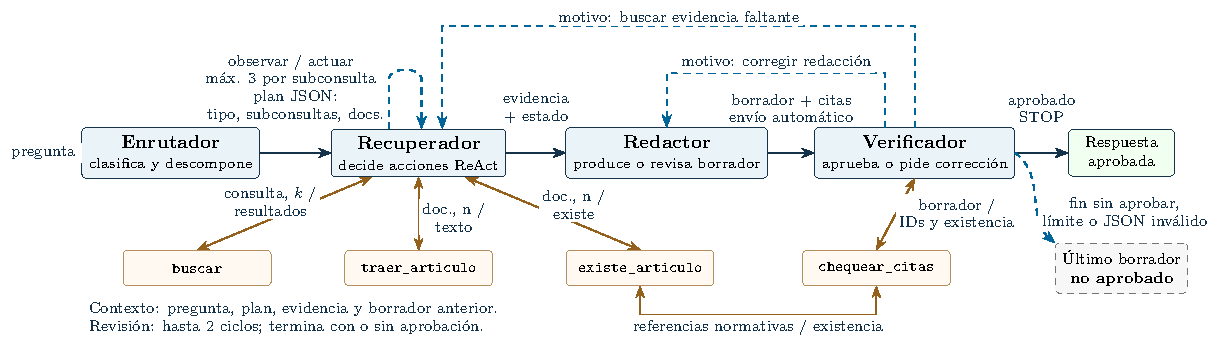
\includegraphics[width=\linewidth]{grafo_compacto.pdf}}
{\fontsize{7}{8}\selectfont\color{gris} Continuas: flujo; discontinuas: revisión/parada; dobles: argumentos y resultados de herramientas. El tipo del Enrutador activa la comprobación de artículos en premisas falsas. E5 recupera evidencia; no es otro modelo agente.}\par
\vspace{2pt}{\color{azul!35}\hrule height .4pt}\vspace{2pt}

\noindent\begin{minipage}[t]{0.486\linewidth}
\fontsize{9}{10.4}\selectfont
\seccion{3. Roles, contratos y técnicas}
Prompts propios en \texttt{prompts/01-04}. Enrutador, Recuperador y Verificador deciden rutas o paradas. El controlador transfiere siempre el borrador del Redactor al Verificador.

\rol{Enrutador.} Pregunta $\to$ JSON \{tipo, sub\_consultas, documentos\}. Clasifica, descompone y fija el modo; entrega el plan. Sin herramientas directas. \textbf{Few-shot}: guía cruces y premisas falsas.

\rol{Recuperador.} Subconsulta, evidencia y observación $\to$ JSON \{accion, args\}, evidencia y estado. Elige \texttt{buscar}, \texttt{traer}, \texttt{existe} o \texttt{suficiente}; hasta tres acciones por subconsulta. \textbf{ReAct}: re-busca según lo observado.

\rol{Redactor.} Pregunta, modo, evidencia y objeciones $\to$ Respuesta / Condiciones / Fuente. Redacta, corrige o declara falta de respaldo; sin herramientas directas. \textbf{CoT por prompt}: aborda cálculos y excepciones; se retira el razonamiento de la respuesta visible.

\rol{Verificador.} Pregunta, borrador, evidencia y \texttt{chequear\_citas} $\to$ JSON \{aprobado, destino, motivo\}. Aprueba o devuelve objeciones al Redactor o Recuperador. \textbf{Self-refine con criterios}: revisa suficiencia y citas.

\textbf{División del trabajo.} Planificar determina qué buscar; recuperar reúne respaldo; redactar responde; verificar aplica criterios en otra llamada. Permite corregir la fase necesaria, pero no garantiza independencia entre llamadas al mismo modelo.

\seccion{4. Ablaciones y alcance}
\textbf{Sin few-shot:} elimina ejemplos del Enrutador. \textbf{Sin CoT:} elimina la instrucción del Redactor; el Verificador la conserva. \textbf{Sin ReAct:} elimina ciclo y llamadas del Recuperador, manteniendo la búsqueda base. \textbf{Sin Verificador:} toma el primer borrador de v6 desde las trazas; no es otra corrida GPU. Las dos últimas eliminan componentes completos.

Mismos conjuntos y pauta por condición. La semilla depende del prompt: cambiarlo altera también el muestreo. Hay una corrida por condición; diferencias de uno o dos aciertos no prueban ventajas estables. Las preguntas se usaron durante desarrollo, por lo que no se demuestra generalización.
\end{minipage}\hfill
\begin{minipage}[t]{0.486\linewidth}
\fontsize{9}{10.4}\selectfont
\seccion{5. Resultados y contribuciones}
Corrección externa propuesta con Claude según la pauta de D2 y motivos por fila; \textbf{nueve casos v6 siguen en revisión}. Se evalúa el texto final, aunque no tenga aprobación interna.

{\fontsize{8.2}{9.6}\selectfont\setlength{\tabcolsep}{3pt}
\renewcommand{\arraystretch}{1.08}
\begin{tabularx}{\linewidth}{@{}Xccc@{}}
\toprule
\textbf{Configuración} & \textbf{Base (50)} & \textbf{Dif. (25)} & \textbf{Llam.}\\
\midrule
Directo & 1 (2\%) & 0 (0\%) & 1\\
RAG D2 & 40 (80\%) & 16 (64\%) & 1\\
\rowcolor{suave}\textbf{Completo v6} & \textbf{46 (92\%)} & \textbf{20 (80\%)} & \textbf{9,5}\\
Sin few-shot & 44 (88\%) & 19 (76\%) & 10,7\\
Sin ReAct & 45 (90\%) & 18 (72\%) & 3,9\\
Sin CoT (Redactor) & 46 (92\%) & 19 (76\%) & 8,3\\
Sin Verificador & 44 (88\%) & 19 (76\%) & 6,4\\
\bottomrule
\end{tabularx}}
{\fontsize{7}{8}\selectfont\color{gris} Aciertos (porcentaje). Llam.: media de llamadas al modelo por pregunta, sobre 75 entradas; excluye herramientas automáticas.}\par

Frente a D2: \textbf{7 mejoras y 1 regresión} en las originales (+12 puntos porcentuales); \textbf{6 mejoras y 2 regresiones} en las difíciles (+16 puntos).

Sin ReAct se pierden dos aciertos difíciles; H05 queda sin evidencia para calcular. Sin few-shot, las clasificaciones de premisa falsa bajan de 14 a 6. Sin CoT se empata en las originales y el tiempo medio baja de 110 a 55 s. Verificar añade tres aciertos netos sobre 75 respecto del primer borrador, con una regresión en H07.

\seccion{6. Fallo, costo y límites}
\textbf{H03: días entre inicio de clases y modificación.} Faltan fechas entre las seis evidencias; el Redactor inventa 31 y 262 días. El Verificador rechaza, pero la revisión y re-búsqueda no resuelven la carencia: termina \textbf{no aprobado tras 19 llamadas}. Traza: \texttt{resultados\_v6/trazas\_D3.json}, clave \texttt{dificil\_25:H03}.

\textbf{Aprobar no equivale a acertar:} siete de 64 aprobaciones son incorrectas; nueve aciertos son borradores rechazados. El Verificador recibe hasta 700 caracteres por unidad; comprobar citas no garantiza respaldo semántico. Costo de v6: \textbf{711 llamadas / 75} = 9,48 y 110 s por pregunta en T4.

\seccion{7. Reproducción y trazabilidad}
\href{\REPO}{\texttt{D3 alvaro/README.md}} enlaza Colab, prompts, CSV, planillas y trazas por entrada. \texttt{Demo\_D3.ipynb} muestra mensajes de una consulta y permite inspeccionar H03 histórico. \texttt{auditar.py} verifica hashes y correspondencia CSV/trazas. Se conserva el ZIP original; el entorno se registra, sin garantizar identidad con versiones históricas no fijadas.
\end{minipage}
\end{document}
